\section{Domande del Syllabus}

\subsection{Precisione di macchina}
Si parte da un numero reale, scritto in notazione floating point:\\
\begin{displaymath}
    x=sign(x)(0,d_1d_2....dt...)\cdot b^p
\end{displaymath}
È importante tenere a mente che la 1° cifra dopo la virgola $(d_1)$ è diversa da zero.\\
Quindi si scrive il numero arrotondato a $t$ cifre di mantissa, e si scrive la definizione formale di \underline{arrotondamento}.\\
Poi diciamo che la precisione di macchina è l'errore relativo di arrotondamento, e scriviamo l'errore di arrotondamento:
\begin{displaymath}
    \frac{|x-fl^t(x)|}{|x|},  |x| \neq 0
\end{displaymath}
Quindi stimiamo questo rapporto in due parti: prima il numeratore.\\
Le cifre dei due numeri sono uguali fino alla $t-1$, cambia dalla $t$ in poi (per l'arrotondamento), e con un esempio di può vedere che questa quantità è $\leq \frac{b^{-t}}{2}$\\
ESEMPIO: se $x=3.14$ e voglio arrotondare ai decimi, l'errore che compio è $\leq$ mezzo decimo (in questo caso di 0.04):\\
\begin{center}
    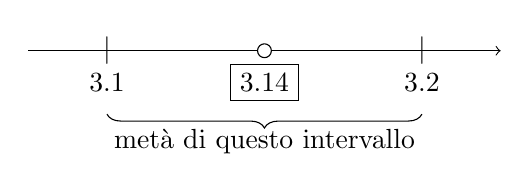
\begin{tikzpicture}
    % Retta orientata
    \draw[->] (0,0) -- (6,0);
    
    % Numeri sotto la retta
    \node at (1,-0.4) {$3.1$};
    \node[draw] at (3,-0.4) {$3.14$};
    \node at (5,-0.4) {$3.2$};
    
    % Numeri sulla retta
    \node at (1,0) {$|$};
    \node[draw, circle, fill=white, inner sep=0pt, minimum width=5pt] at (3,0) {};
    \node at (5,0) {$|$};
    
    % Parentesi graffa orizzontale
    \draw[decorate,decoration={brace,amplitude=5pt,mirror},xshift=0pt,yshift=-3pt] (1,-0.7) -- (5,-0.7) node[midway,below,yshift=-2pt] {metà di questo intervallo};
    \end{tikzpicture}
\end{center}
Ora stimiamo il denominatore. Sappiamo che è una quantità positiva (c'è il valore assoluto), è $\neq$ 0, e la prima cifra decimale $(d_1)$ deve essere diversa da zero. Questo serve ad evitare che ci siano più rappresentazioni dello stesso numero.\\
Quindi $|x|$ è almeno $(\geq)$ $0.1 \cdot b^p$ (non ci serve uno specifico p), ovvero $b^{-1}\cdot b^p => b^{p-1}$.\\
Siccome nella definizione di errore relativo $|x|$ "sta sotto", dobbiamo scrivere il reciproco: 
\begin{displaymath}\frac{1}{|x|}\leq \frac{1}{b^{p-1}}\end{displaymath}
Da notare il fatto che è cambiato il verso della disequazione.\\
Quindi uniamo i due pezzi, e otteniamo che:\\
\begin{center}
    \large\begin{displaymath}
        \frac{|x-fl^t(x)|}{|x|}\leq \frac{\frac{b^{-t}}{2}}{b^{p-1}}= \frac{b^{p-t+1-p}}{2}= \frac{b^{1-t}}{2}
    \end{displaymath}
\end{center}
Che è la nostra precisione di macchina.
\newpage

\subsection{Stabilità delle operazioni}
Questa è la più lunga di tutte le dimostrazioni, ma:
\begin{itemize}
    \item all'esame il prof ne chiede sempre metà (solitamente moltiplicazione e divisione oppure somma algebrica)
    \item Non serve impararsi tutto a memoria: gran parte del testo sono operazioni algebriche. Si utilizza la diseguaglianza triangolare e si moltiplica/divide per una certa quantità (questo nel caso della somma algebrica, nella moltiplicazione si somma/sottrae).
    \item Si inizia dalla definizione, ovvero l'errore relativo che ho su un'operazione con numeri approssimati:\begin{displaymath}\varepsilon _{x\star y}=\frac{|x\star y - \widetilde{x}\star \widetilde{y}|}{|x \star y|} \end{displaymath}  Dove al posto di $\star$ si mette una delle operazioni, e $\widetilde{x}$, $\widetilde{y}$ (con la tilde) sono i numeri approssimati.
    \item La sottrazione (ovvero la somma algebrica nel caso in cui il segno dei due numeri è diverso) è l'unica operazione instabile (quando $x$ e $y$ sono vicini in termini relativi)
\end{itemize}

\newpage
\subsection{Convergenza del metodo di bisezione}
Questa è la prima domanda in cui il prof inizia a utilizzare la lettera $\xi$ (csi), che semplicemente indica la soluzione che stiamo cercando. Invece con $x$ (oppure $x_n$) indica la "soluzione" che abbiamo trovato a una certa iterazione. In generale, più iterazioni abbiamo e più la nostra $x$ si avvicina a $\xi$.\\
Con \underbar{convergenza} di un metodo (in questo caso la bisezione) si intende il fatto che, facendo iterazioni, ci avviciniamo sempre di più alla soluzione $\xi$, lo "zero" della funzione.\\
Il metodo di bisezione funziona applicando iterativamente il \underbar{teorema degli zeri} (o teorema di Bolzano).
\begin{center}
    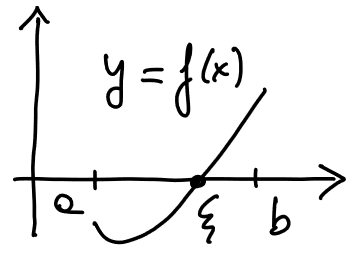
\includegraphics[scale=0.6]{./res/img/bisezione1.png}
\end{center}
Se ho una funzione continua in un intervallo $[a,b]$ e $f(a) \cdot f(b)\leq 0$ (ovvero hanno segno opposto), allora esiste un punto $\xi$, con $f(\xi)=0$, che appartiene all'intervallo $(a,b)$.\\
Il metodo consiste nell'individuare il punto medio, e continuare il procedimento sulla metà dell'intervallo in cui vale la condizione che i due estremi hanno segno opposto.\\
Esempio:
\begin{center}
    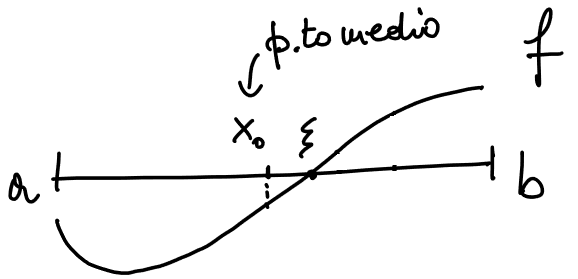
\includegraphics[scale=0.6]{./res/img/bisezione2.png}
\end{center}
In questa funzione abbiamo come estremi $a, b$. Individuiamo il \underbar{punto medio} $x_0$, e la successiva iterazione la facciamo sul semintervallo $[a,x]$, perché $f(a) f(x_0)\leq 0$.\\
Il punto medio è $x_n=\frac{a_n+b_n}{2}$.\\
Poi si individuano tre successioni: ${a_n}$, ${b_n}$, ${x_n}$, tali che:
\begin{itemize}
    \item $|\xi-a_n|\leq b_n-a_n = \frac{b-a}{2^n}$
    \item $|\xi-b_n|\leq b_n-a_n = \frac{b-a}{2^n}$
    \item $|\xi-x_n|\leq \frac{b_n-a_n}{2} = \frac{b-a}{2^{n+1}}$
\end{itemize}
$\frac{b-a}{2^n}$ è la lunghezza dell'intervallo $b_n-a_n$, mentre $\frac{b-a}{2^{n+1}}$ è la distanza tra il punto medio e $\xi$, e non può superare metà dell'intervallo $b_n-a_n$.\\
Quindi si dimostra che le tre successioni convergono ad uno zero, utilizzando il teorema dei carabinieri:\\
\begin{displaymath}
    0 \leq |\xi-a_n|, |\xi-b_n| < \frac{b-a}{2^n}\to 0, n \to \infty \overset{teor. carabinieri}{\implies} |\xi-a_n|, |\xi-b_n| \to 0, n \to \infty
\end{displaymath}
Qui semplicemente dichiamo che $|\xi-a_n|, |\xi-b_n|$ sono due quantità positive (per via dei valori assoluti), e da quello che abbiamo detto prima sono $\leq$ di $ \frac{b-a}{2^n}$.\\
Calcolando il $\lim_{n\to \infty} \frac{b-a}{2^n}$ otteniamo che è zero. Quindi possiamo utilizzare il teorema dei carabinieri per dire che le due successioni tendono a zero.\\
Lo stesso ragionamento lo utilizziamo per la terza successione:
\begin{displaymath}
    0 \leq |\xi-x_n|< \frac{b-a}{2^{n+1}}\implies |\xi-x_n| \to 0, n\to \infty
\end{displaymath}